%***************************************PREAMBLE***************************************
\documentclass[a4paper,12pt]{article}

\usepackage[utf8]{inputenc}
\usepackage[margin=0.7in]{geometry}
\usepackage[T1]{fontenc}
\usepackage{graphicx}
\usepackage{float}
\usepackage{setspace}
\usepackage{appendix}
\usepackage{amsmath}
\usepackage{cite}
\usepackage{caption}
\usepackage{subcaption}


%***************************************DOCUMENT***************************************

\DeclareMathOperator*{\argmin}{\arg\!\min}
\DeclareMathOperator*{\argmax}{\arg\!\max}

\graphicspath{ {./images/} }
\setlength{\parindent}{0pt}

\begin{document}
	\fontfamily{ptm}\selectfont
	%%%%%%%%%%%%%%%%%%%%%%%%%%%%%%%%%%%%%%%COVERSHEET%%%%%%%%%%%%%%%%%%%%%%%%%%%%%%%%%%%%%%%
	\begin{titlepage}
		\setlength{\voffset}{-0.8in}
		\noindent \makebox[\textwidth]{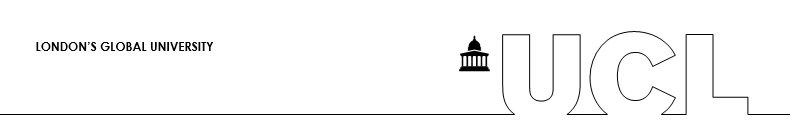
\includegraphics[width=1.2\textwidth]{Coversheet_Header.png}}
	
			\vspace{15mm}
			
			\begin{center}
				{\Huge \textbf{COMP0037 \\ \vspace{10mm} Report}}
			
				\vspace{8mm}
			
				\begin{spacing}{1.8}
					{\huge Learning and Planning}
				\end{spacing}
		
			
				\vspace{12mm}
			
				{\LARGE \textbf{Group AS}}
				
				\vspace{10mm}
				
				\begin{tabular}{ll}
					\underline{\textbf{Student Name}}  & \hspace{4mm} \underline{\textbf{Student number}} \vspace{2mm} \\
					Arundathi Shaji Shanthini & \hspace{4mm} 16018351 \\ 
					Dmitry Leyko & \hspace{4mm}  16021440\\ 
					Tharmetharan Balendran & \hspace{4mm} 17011729\\ 
				\end{tabular}
				
				\vspace{13mm}
				
				\begin{tabular}{ll}
					\textbf{Department:} &  Department of Electronic and Electrical Engineering\\ \vspace{3mm}
					\textbf{Submission Date:} &  28\textsuperscript{th} of April 2020
				\end{tabular}
			\end{center}
	\end{titlepage}
	%%%%%%%%%%%%%%%%%%%%%%%%%%%%%%%%%%%%%%
	
	\pagebreak
	
	\tableofcontents
	
	\pagebreak
	
	%%%%%%%%%%% PART 1 %%%%%%%%%%%%%%%%%
	\section{Decision Re-Plan Policy}

		\subsection{Policy Selection when Obstacle is Observed}
			
			\begin{figure}[H]
				\centering
				\begin{subfigure}{.4\textwidth}
					\centering
					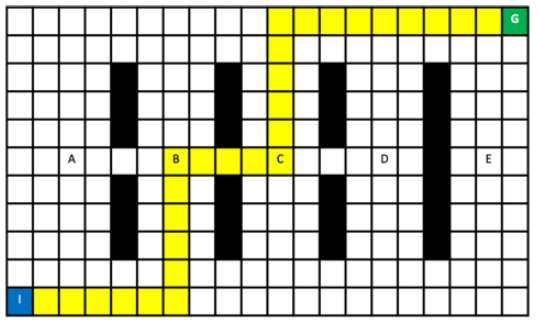
\includegraphics[width=\linewidth]{originalPlannedPath.png}
					\caption{The original planned path form I to G going through Aisle B and C.}
					\label{fig:originalPlannedPath}
				\end{subfigure}
				\begin{subfigure}{.4\textwidth}
					\centering
					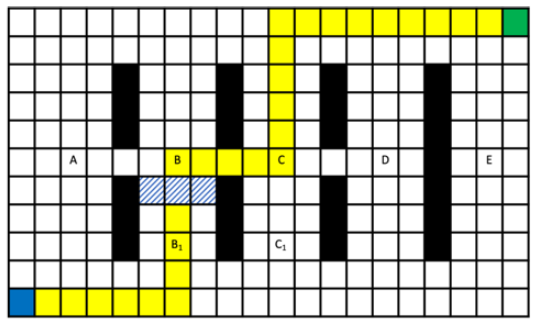
\includegraphics[width=\linewidth]{blockedAisleB.png}
					\caption{An obstacle in aisle B obstructs the planned path of the robot.}
					\label{fig:blockedAisleB}
				\end{subfigure}
				\caption{Illustration of case where robot observes an obstruction to it's planned path.}
				\label{fig:task1_1Figures}
			\end{figure}

			The scenario that we will be analysing is the case shown in Fig. \ref{fig:originalPlannedPath}. The robot is required to go from a cell $I$ to a cell $G$. These cells are marked blue and green in Fig. \ref{fig:originalPlannedPath} respectively. The figure also shows the original planned path that the robot computed going down aisle B. However, once the robot turns into aisle B it observes that the aisle is blocked. This observation is done at the point when the robot reaches the cell labelled $B_{1}$. At this point the robot can either decide to wait until the obstruction clears or it can re-plan a path. Once the robot observes the obstacle, the time the robot must wait for the obstacle to clear may be represented by the expression in Eq. \ref{eq:waitTime}. 

			\begin{equation}
				T=\frac{0.4}{\lambda_{B}}+\widetilde{T}
				\label{eq:waitTime}
			\end{equation}

			The wait time is dependent on $\lambda_{B}$ and a random variable $\widetilde{T}$. The random variable $\widetilde{T}$ is sampled from a exponential distribution with a rate parameter of $0.5\lambda_{B}$. The probability density function (PDF) for $\widetilde{T}$ is shown in Eq. \ref{eq:waitTimePDF}. 

			\begin{equation}
				f(t) = \left\{
				\begin{array}{ll}
					0.5\lambda_{B} e^{-0.5\lambda_{B} t} & \quad t \geq 0 \\
					0 & \quad t < 0
				\end{array}
				\right.
				\label{eq:waitTimePDF}
			\end{equation}

			As previously mentioned, the robot has two options to choose from: to wait for the obstacle to clear, or to re-plan and execute the new path. The two are different policies the robot must choose from. We use the symbol $\pi$ to denote a policy. A policy is a mapping from the world state to an action the robot can execute. 

		\subsection{Policy Selection at Start}

		\subsection{Considering the Probability of the Obstacle Being Present}

		\subsection{Considering Multiple Obstacles}

	%%%%%%%%%%%%%%%%%%%%%%%%%%%%%%%%%%%%%%
	
	%%%%%%%%%%% PART 2 %%%%%%%%%%%%%%%%%
	\section{ROS Implementation}

		

	%%%%%%%%%%%%%%%%%%%%%%%%%%%%%%%%%%%%%%
	
	\bibliographystyle{IEEEtran}
	\bibliography{references}

	%%%%%%%%%%%%%%%%%%%%%%%%%%%%%%%%%%%%%%

	\newpage
	\appendix
	\appendixpage
	\addappheadtotoc
	
\end{document}